\documentclass{report}
\usepackage[utf8]{inputenc}

%	Changing document font to Helvetica.
\usepackage[scaled]{helvet}
\renewcommand\familydefault{\sfdefault} 
\usepackage[T1]{fontenc}

%	Changing Margins and other formatting
\usepackage{geometry}
\geometry{
	a4paper,
	total={170mm,257mm},
	left=1.5in,
	top=1in,
	right=1.5in,
	bottom=1in
}
\setlength{\parskip}{1em}

%	Source Code Highlighting
\usepackage{minted}
%	For Console
\setminted[console]{
frame=lines,
framesep=2mm,
baselinestretch=1.2,
fontsize=\footnotesize,
linenos,
breaklines
}
%	For Shell Scripts
\setminted[bash]{
	frame=lines,
	framesep=2mm,
	baselinestretch=1.2,
	fontsize=\footnotesize,
	linenos,
	breaklines
}
%	For HTML Pages
\setminted[html]{
	frame=lines,
	framesep=2mm,
	baselinestretch=1.2,
	fontsize=\footnotesize,
	linenos,
	breaklines
}
%	For HTTP Config Files
\setminted[lighttpd]{
	frame=lines,
	framesep=2mm,
	baselinestretch=1.2,
	fontsize=\footnotesize,
	linenos,
	breaklines
}
%	For XML Files
\setminted[xml]{
	frame=lines,
	framesep=2mm,
	baselinestretch=1.2,
	fontsize=\footnotesize,
	linenos,
	breaklines
}

%	Pretty Tables
\usepackage{booktabs}
\usepackage{array, multirow}

%	Custom column for tables
\newcolumntype{P}[1]{ >{\centering\arraybackslash} m{#1\linewidth} }
\newcolumntype{M}[1]{m{#1\linewidth}}

%	Images Support
\usepackage{graphicx}

%	Support for spaces in file names
\usepackage[space]{grffile}

%	SUPPORT FOR WEIRD CHARACTERS
\DeclareUnicodeCharacter{25CF}{$\bullet$}
\usepackage{pmboxdraw}

%	Ignore Pygments Bugs & Errors
\AtBeginEnvironment{minted}{%
	\renewcommand{\fcolorbox}[4][]{#4}}

%	Auto-generate Outline
\usepackage[hidelinks]{hyperref}
%	Added packages below just for the sake of autocomplete.
\usepackage{minted}
\usepackage{booktabs}

\begin{document}
	\input{"Mod2/chapters/2.6 Configuring Advanced Networking"}
	
	\section{Understanding Network Bridges}
	A network bridge is a device that connects two or more networks to form one extended network. For example, an Ethernet bridge connects two or more LANs to create a unified, extended LAN. Virtual bridges are special purpose network interfaces used in virtualized environments. 
	
	Let us consider that the physical host has a NIC called \verb|eno1|. The entire virtualized network in the diagram then has to communicate with any external networks via this interface. However, they can't all just send their packets to the driver of the NIC. Thus, they need a virtual bridge \verb|virbr0|. There can be multiple virtual bridges too. 
	
	\begin{figure}[H]
		\centering
		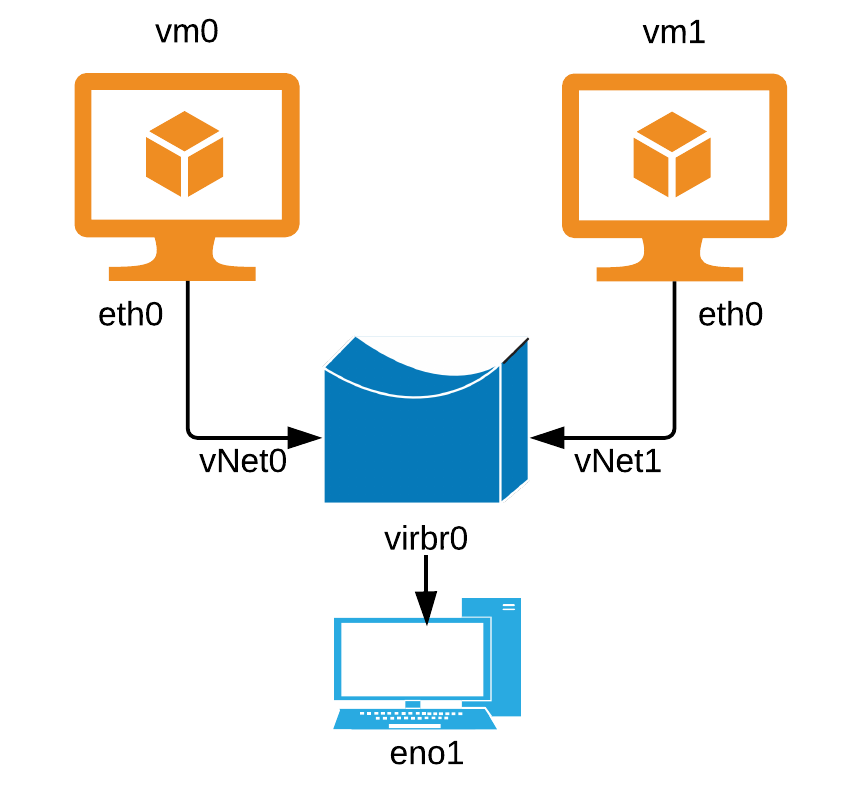
\includegraphics[width=0.5\linewidth]{Mod2/chapters/2.6.b}
		\caption{A virtualized network}
		\label{fig:2}
	\end{figure}
	
	\noindent	
	The virtual bridge acts like a physical switch in the network and merely passes data between the networks. Note that it is incapable of routing decisions. All network traffic - even the traffic that originates from the physical KVM host are handled by it and thus, the virtual bridge decides who can send their packets at a specific moment. 
	
	Each of the virtual machines have their own virtualized Ethernet interface called \verb|eth0| which have to be connected to an interface (port) on the virtual bridge. The virtual bridge names them \verb|vNet0| and \verb|vNet1| accordingly. 
	
	\subsection{Working with Network Bridges}
	
	
	\section{Setting up Network Bridges}
	\section{Understanding Network Bonds and Teams}
	\section{Configuring Network Teams}
	\section{Configuring IPv6} 
	
\end{document}


